\documentclass[12pt,letterpaper]{article}
\usepackage[utf8]{inputenc}
\usepackage{amsmath}
\usepackage{amsfonts}
\usepackage{amssymb}
\usepackage{graphicx}
\usepackage{hyperref}
\usepackage[space]{grffile}
\graphicspath{{/Users/jacob/Documents/My Stuff/Arduino/garmenttransporter/Shirt Stacker/Design/Images/}}

\title{Shirt Stacker}
\author{}
\date{}

\begin{document}
\maketitle
\section{Introduction}
This document describes the shirt-stacking machine which I built. The shirt-stacking machine is capable of picking up shirts from my shirt folder and stacking them. The machine is controlled by an Arduino Robot. All files for the shirt stacker can be found at \url{https://github.com/orangeturtle739/garmenttransporter/tree/master/Shirt\%20Stacker}.

\section{Design}
The shirt stacker consists of a rotating turntable and a spatula. The stacker picks up the shirt on the spatula, rotates and then drops the shirt. The spatula moves up and down using linear bearings. Figure \ref{topview} shows a rendering of the shirt stacker.

A SketchUp model of the shirt folder can be found at \url{https://github.com/orangeturtle739/garmenttransporter/blob/master/Shirt\%20Stacker/Design/Actual%20Design.skp}.

\subsection{Mechanics}
\subsubsection{Rotating}
The rotation is powered by the Arduino Robot's left wheel. The wheel rotates on a rubber track to rotate the shirt stacker. The turntable itself rotates on a lazy susan bearing. The Arduino Robot is attached to the rotating section with a wooden arm. Fiqure \ref{crossection} shows the mechanics.

\subsubsection{Lifting}
The lifting is powered by the Arduino Robot's right wheel. The wheel is attached to a wooden dowel which is attached to a string. When the wheel turns, the string winds up on the dowel. The spool and wheel connection are shown in figure \ref{spool}. The string then passes through a setup consisting of 9 pulleys. The pulleys are visible in figure \ref{pulleys}. This setup lifts the carriage that contains the spatula.

The carriage moves up and down on two linear bearings. Figure \ref{linearbearings} shows the bearings.

\subsubsection{Dumping}
Once the shirt folder has lifted the shirt and rotated to the proper location, the shirt folder drops the shirt. It does this by rotating the spatula. The spatula is attached to a wooden dowel which goes through a bearing. Along the diameter of the flat side of the dowel sticking out of the bearing, there are two nails, both very close to the edge. Figure \ref{nails} shows the location of the nails. Both nails are a attached to a piece of elastic to make the spatula self-righting. One nail is a attached to a string. The other end of the string is tied onto a screw eye on the base of the rotating platform. When the spatula reaches a specific height, this piece of string causes it to rotate. Once the robot lowers the spatula, the elastic makes it level again. This is shown in figure \ref{dumping}.

\section{Parts}
For the lazy susan bearing, I used this part: \url{http://www.amazon.com/gp/product/B00004YOKA/ref=oh_details_o02_s01_i03?ie=UTF8&psc=1}. For the linear bearings, I used these bearings: \url{http://www.amazon.com/gp/product/B00CGR8WUU/ref=oh_details_o03_s00_i01?ie=UTF8&psc=1}. I put the bearings on these shafts: \url{http://www.amazon.com/gp/product/B002BBJ0CA/ref=oh_details_o02_s00_i01?ie=UTF8&psc=1}. I held the shafts in place with these parts: \url{http://www.amazon.com/gp/product/B00C4PBMMY/ref=oh_details_o03_s00_i00?ie=UTF8&psc=1}.

\section{Use}
To use the shirt stacker, install the program which can be found at \url{https://github.com/orangeturtle739/garmenttransporter/blob/master/Shirt\%20Stacker/Code/Code.ino}. After installing the program, turn the Arduino Robot on. Use the Arduino Robot's buttons to control where the shirt stacker will place the shirt. After a button has been pressed, the robot will wait 14 seconds. Then, it will lift the shirt, rotate and then drop the shirt. 

\begin{figure}[ht]
  \centering
    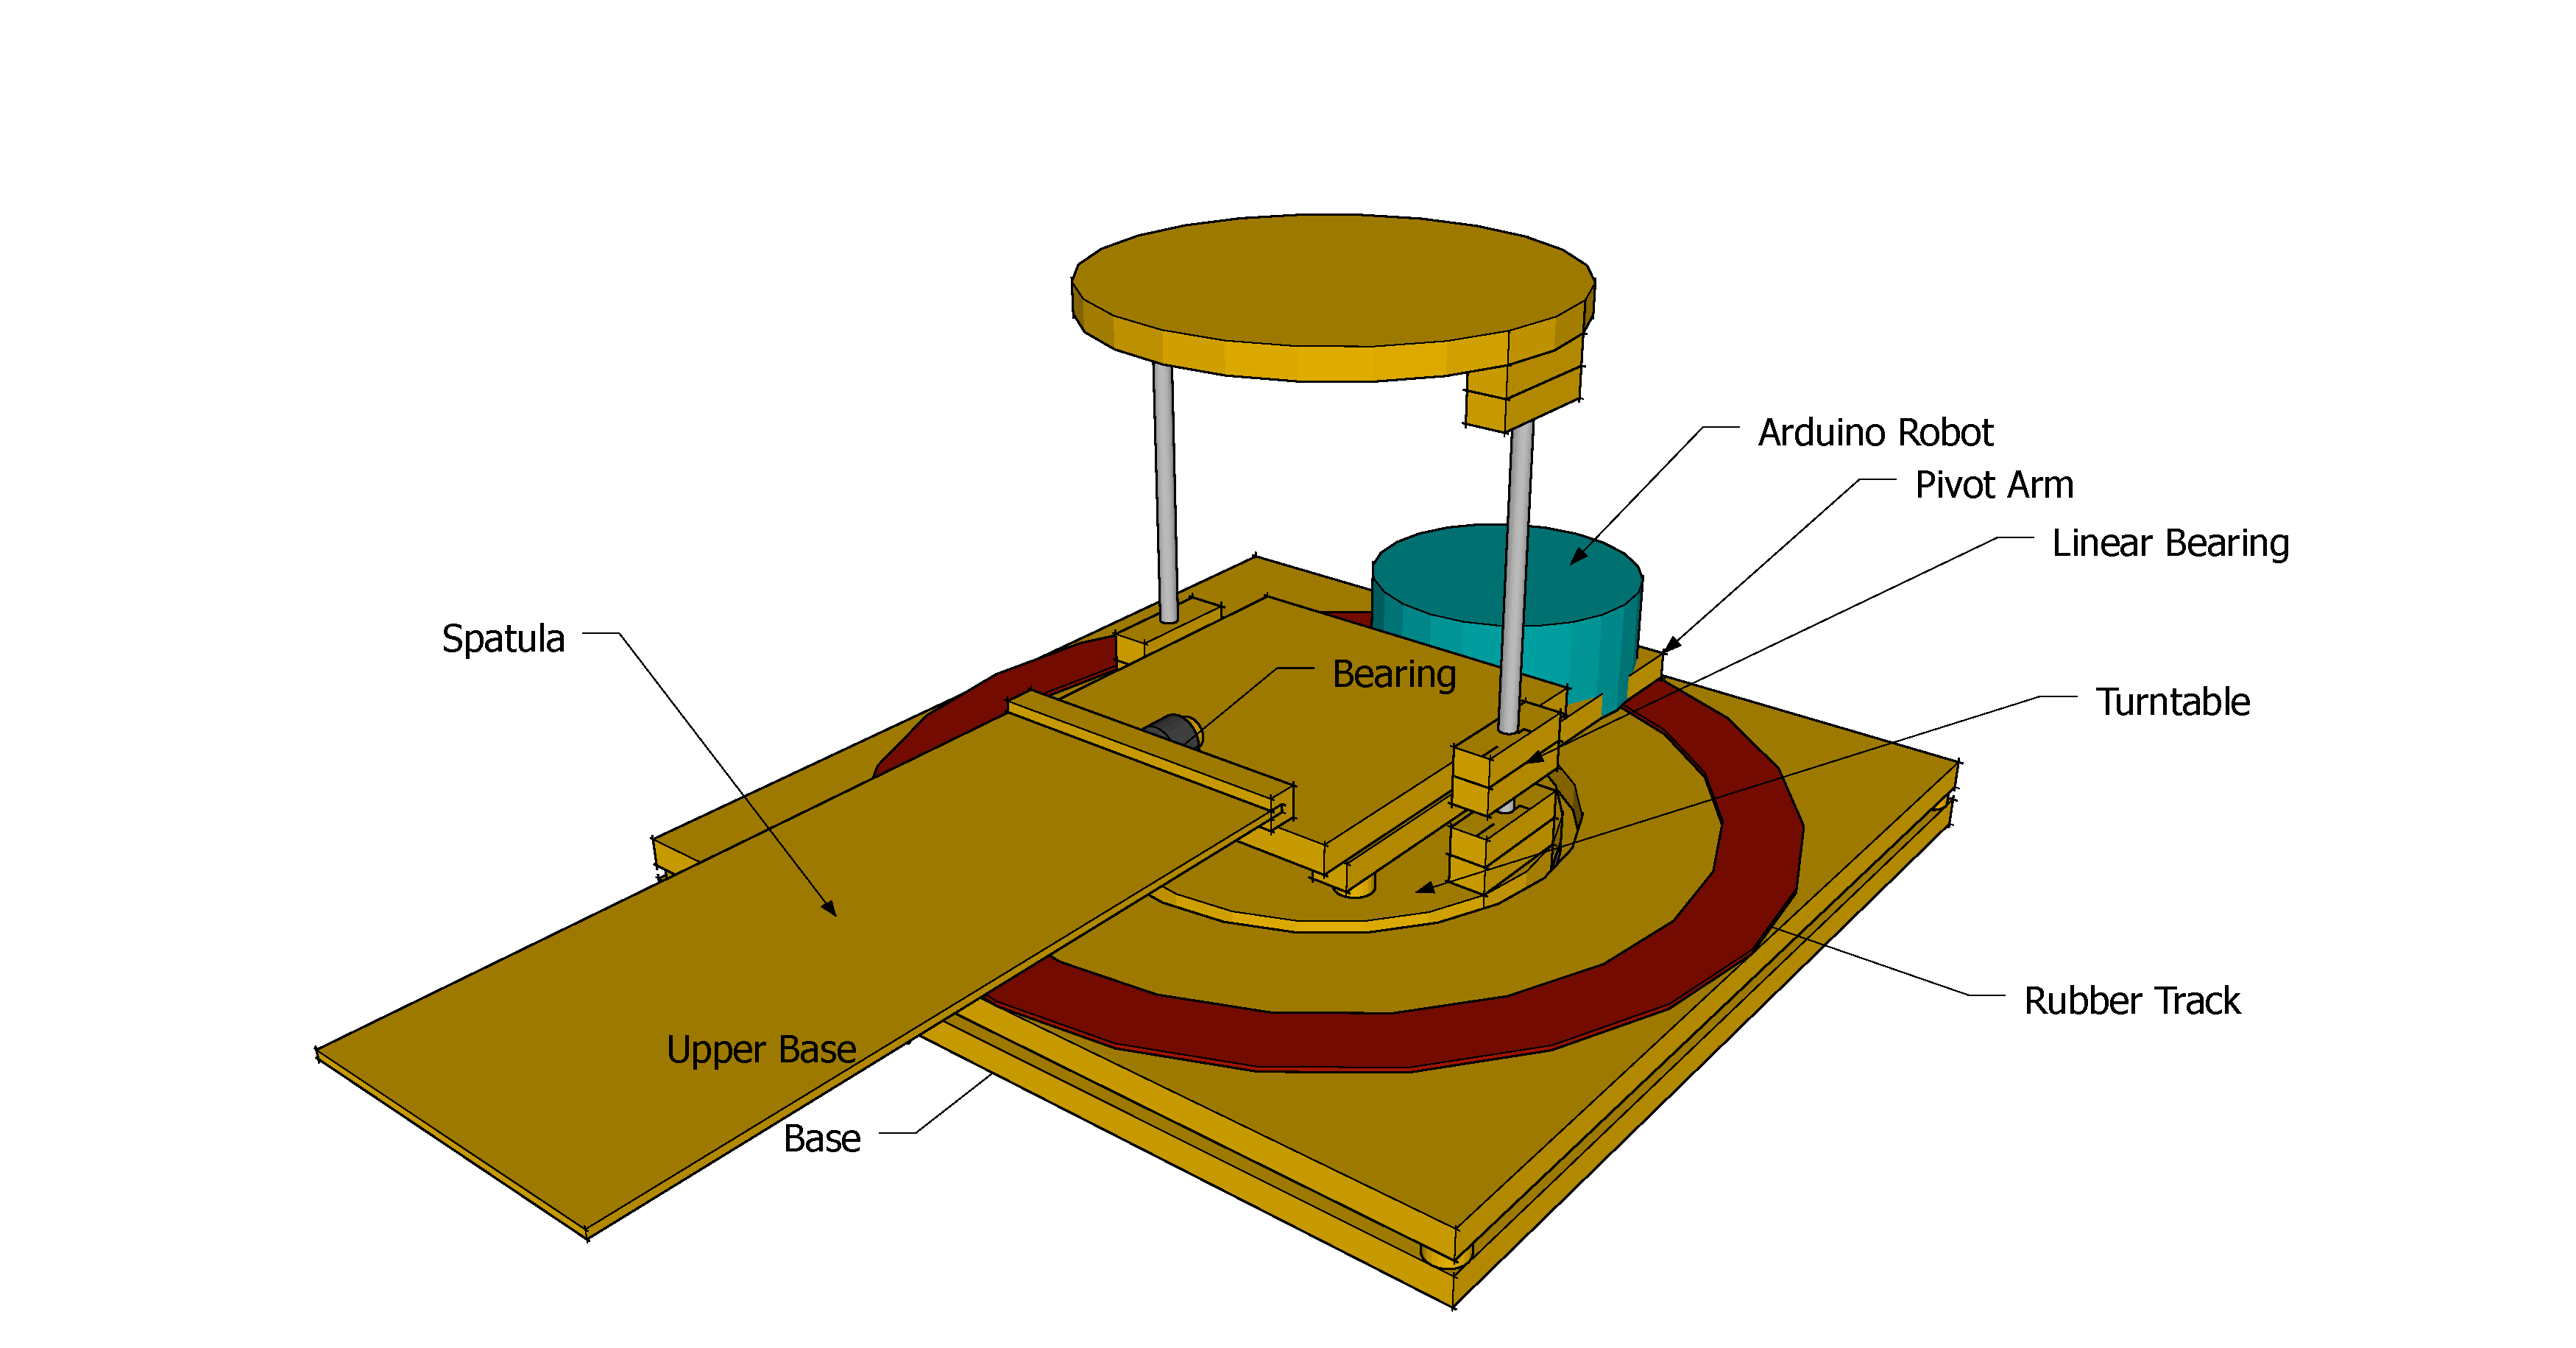
\includegraphics[width=\columnwidth]{Top View.pdf}
    \caption{Top view of shirt stacker.}
    \label{topview}
\end{figure}
\begin{figure}[ht]
  \centering
    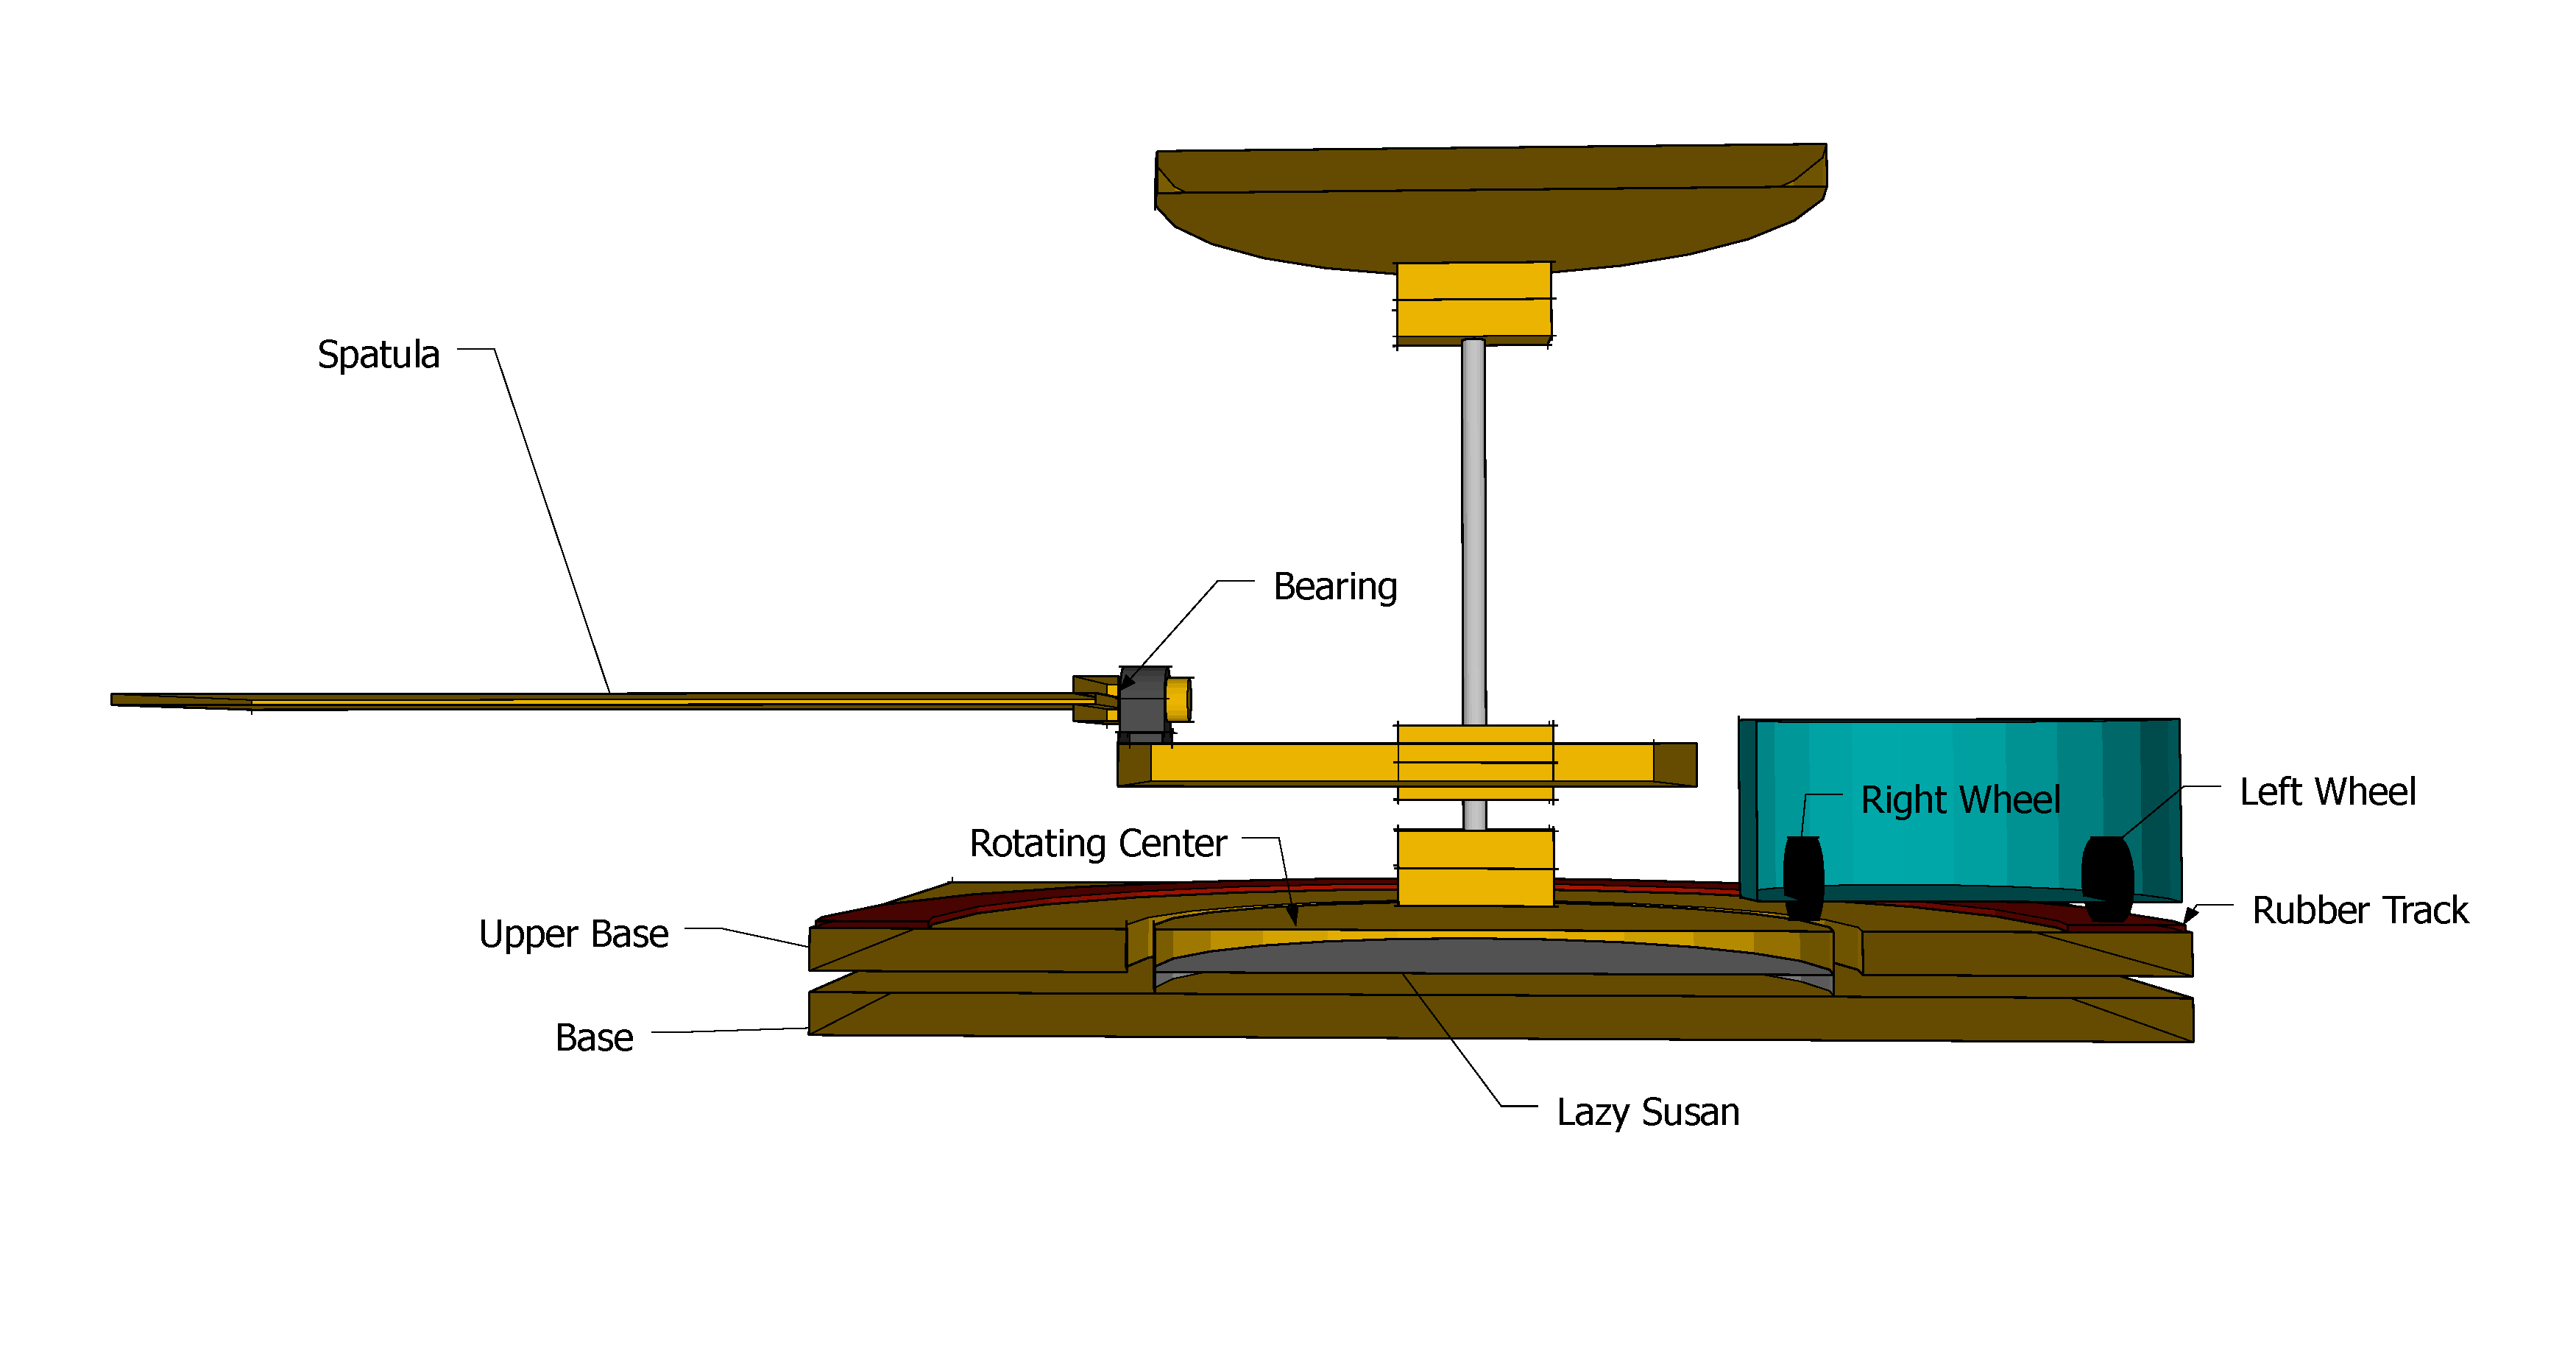
\includegraphics[width=\columnwidth]{Cross Section.pdf}
    \caption{Cross-sectional view of the shirt stacker.}
    \label{crossection}
\end{figure}
\begin{figure}[ht]
  \centering
    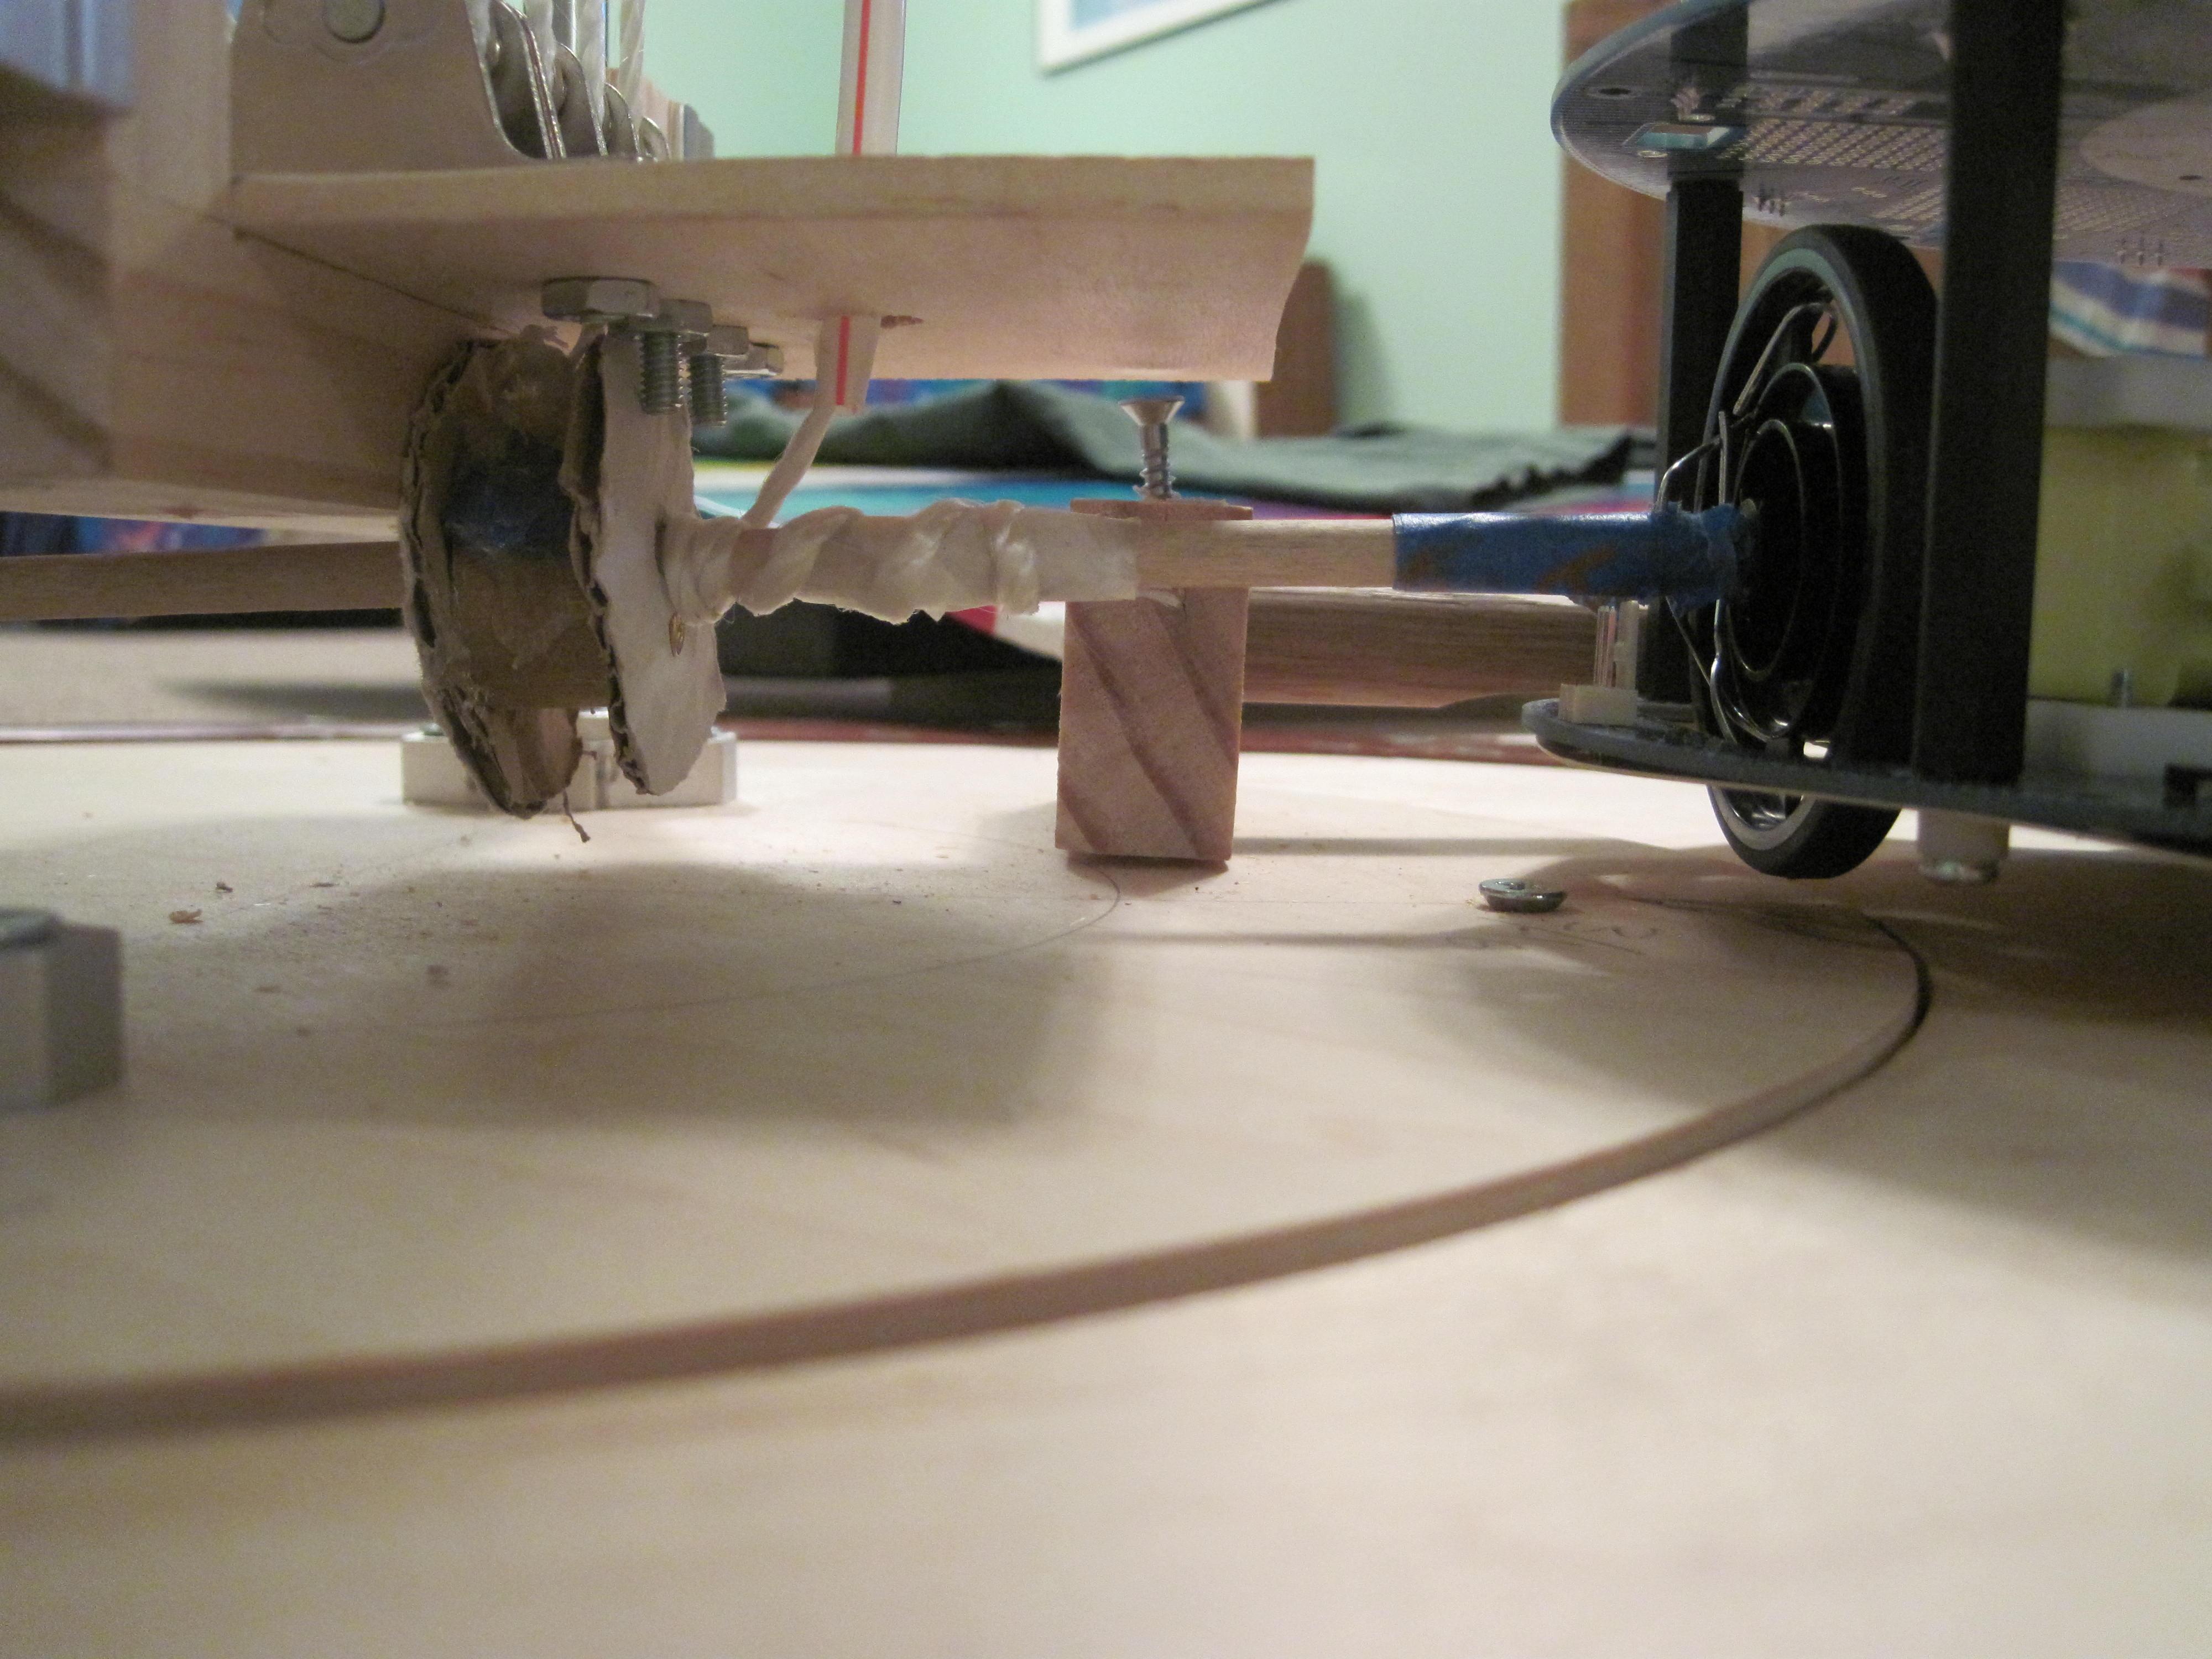
\includegraphics[width=\columnwidth]{Spool.jpg}
    \caption{The spool connected to the right wheel.}
    \label{spool}
\end{figure}
\begin{figure}[ht]
  \centering
    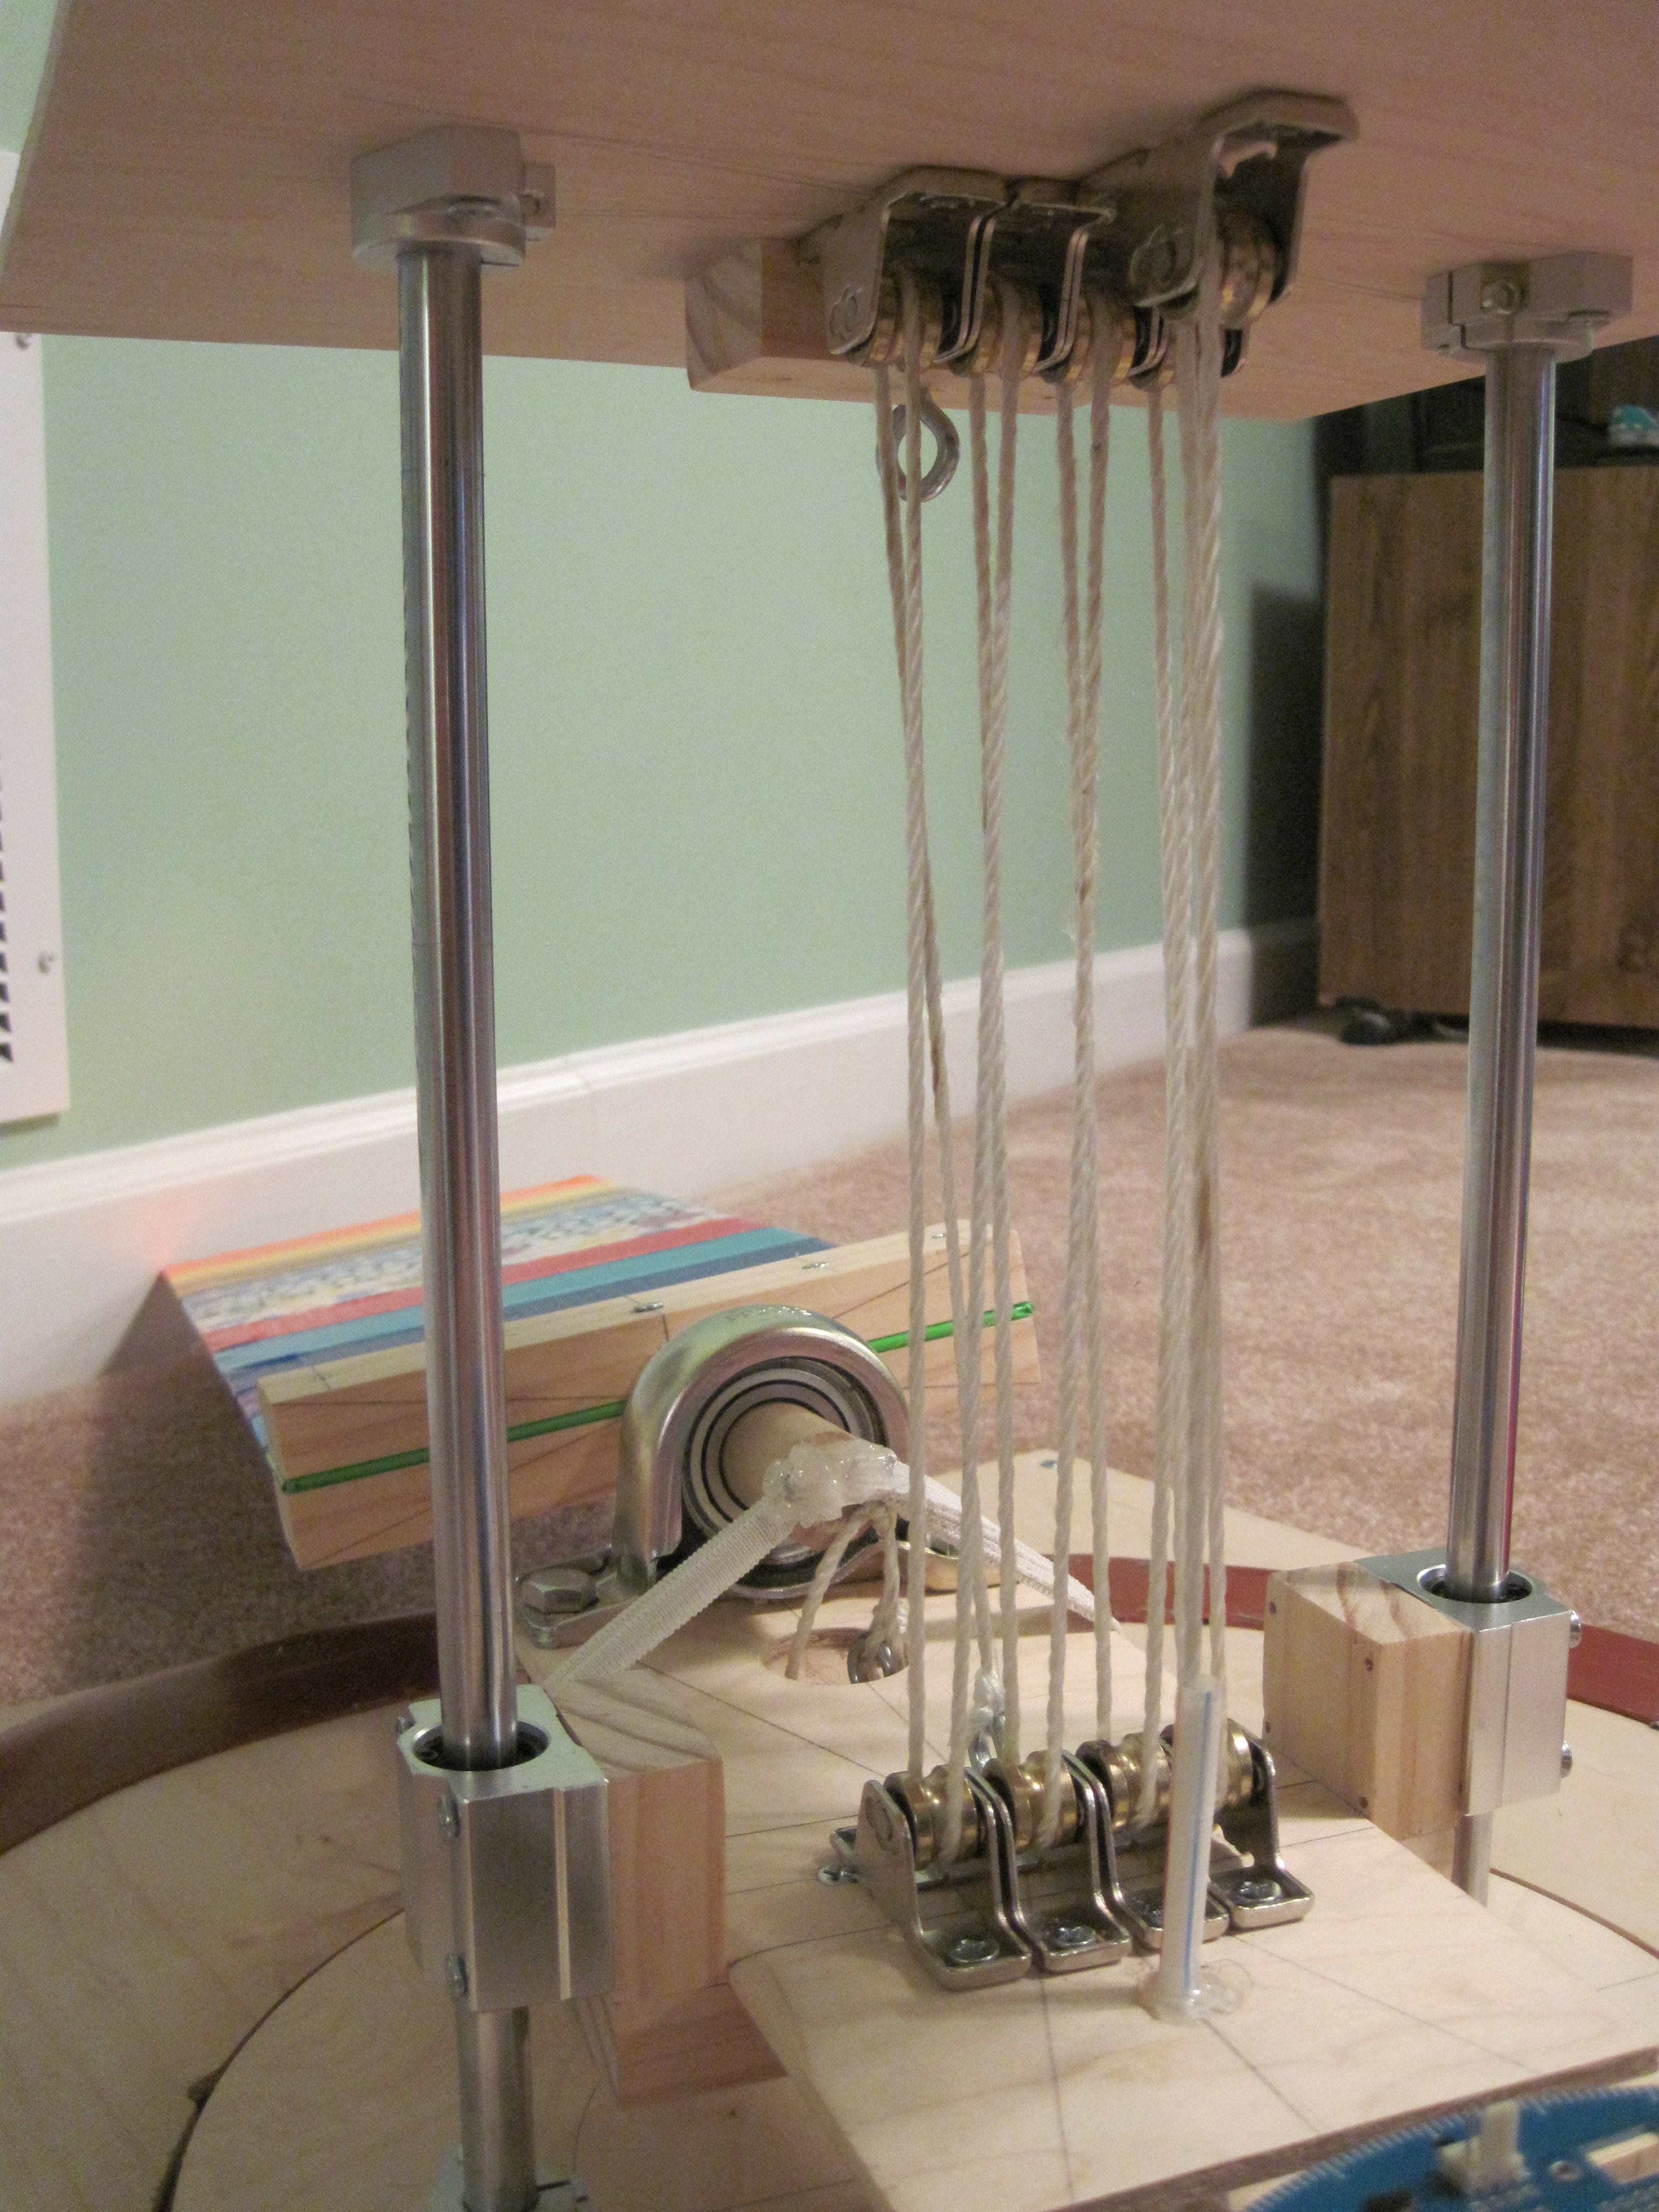
\includegraphics[width=\columnwidth]{Pulleys.jpg}
    \caption{The pulleys on the shirt stacker.}
    \label{pulleys}
\end{figure}
\begin{figure}[ht]
  \centering
    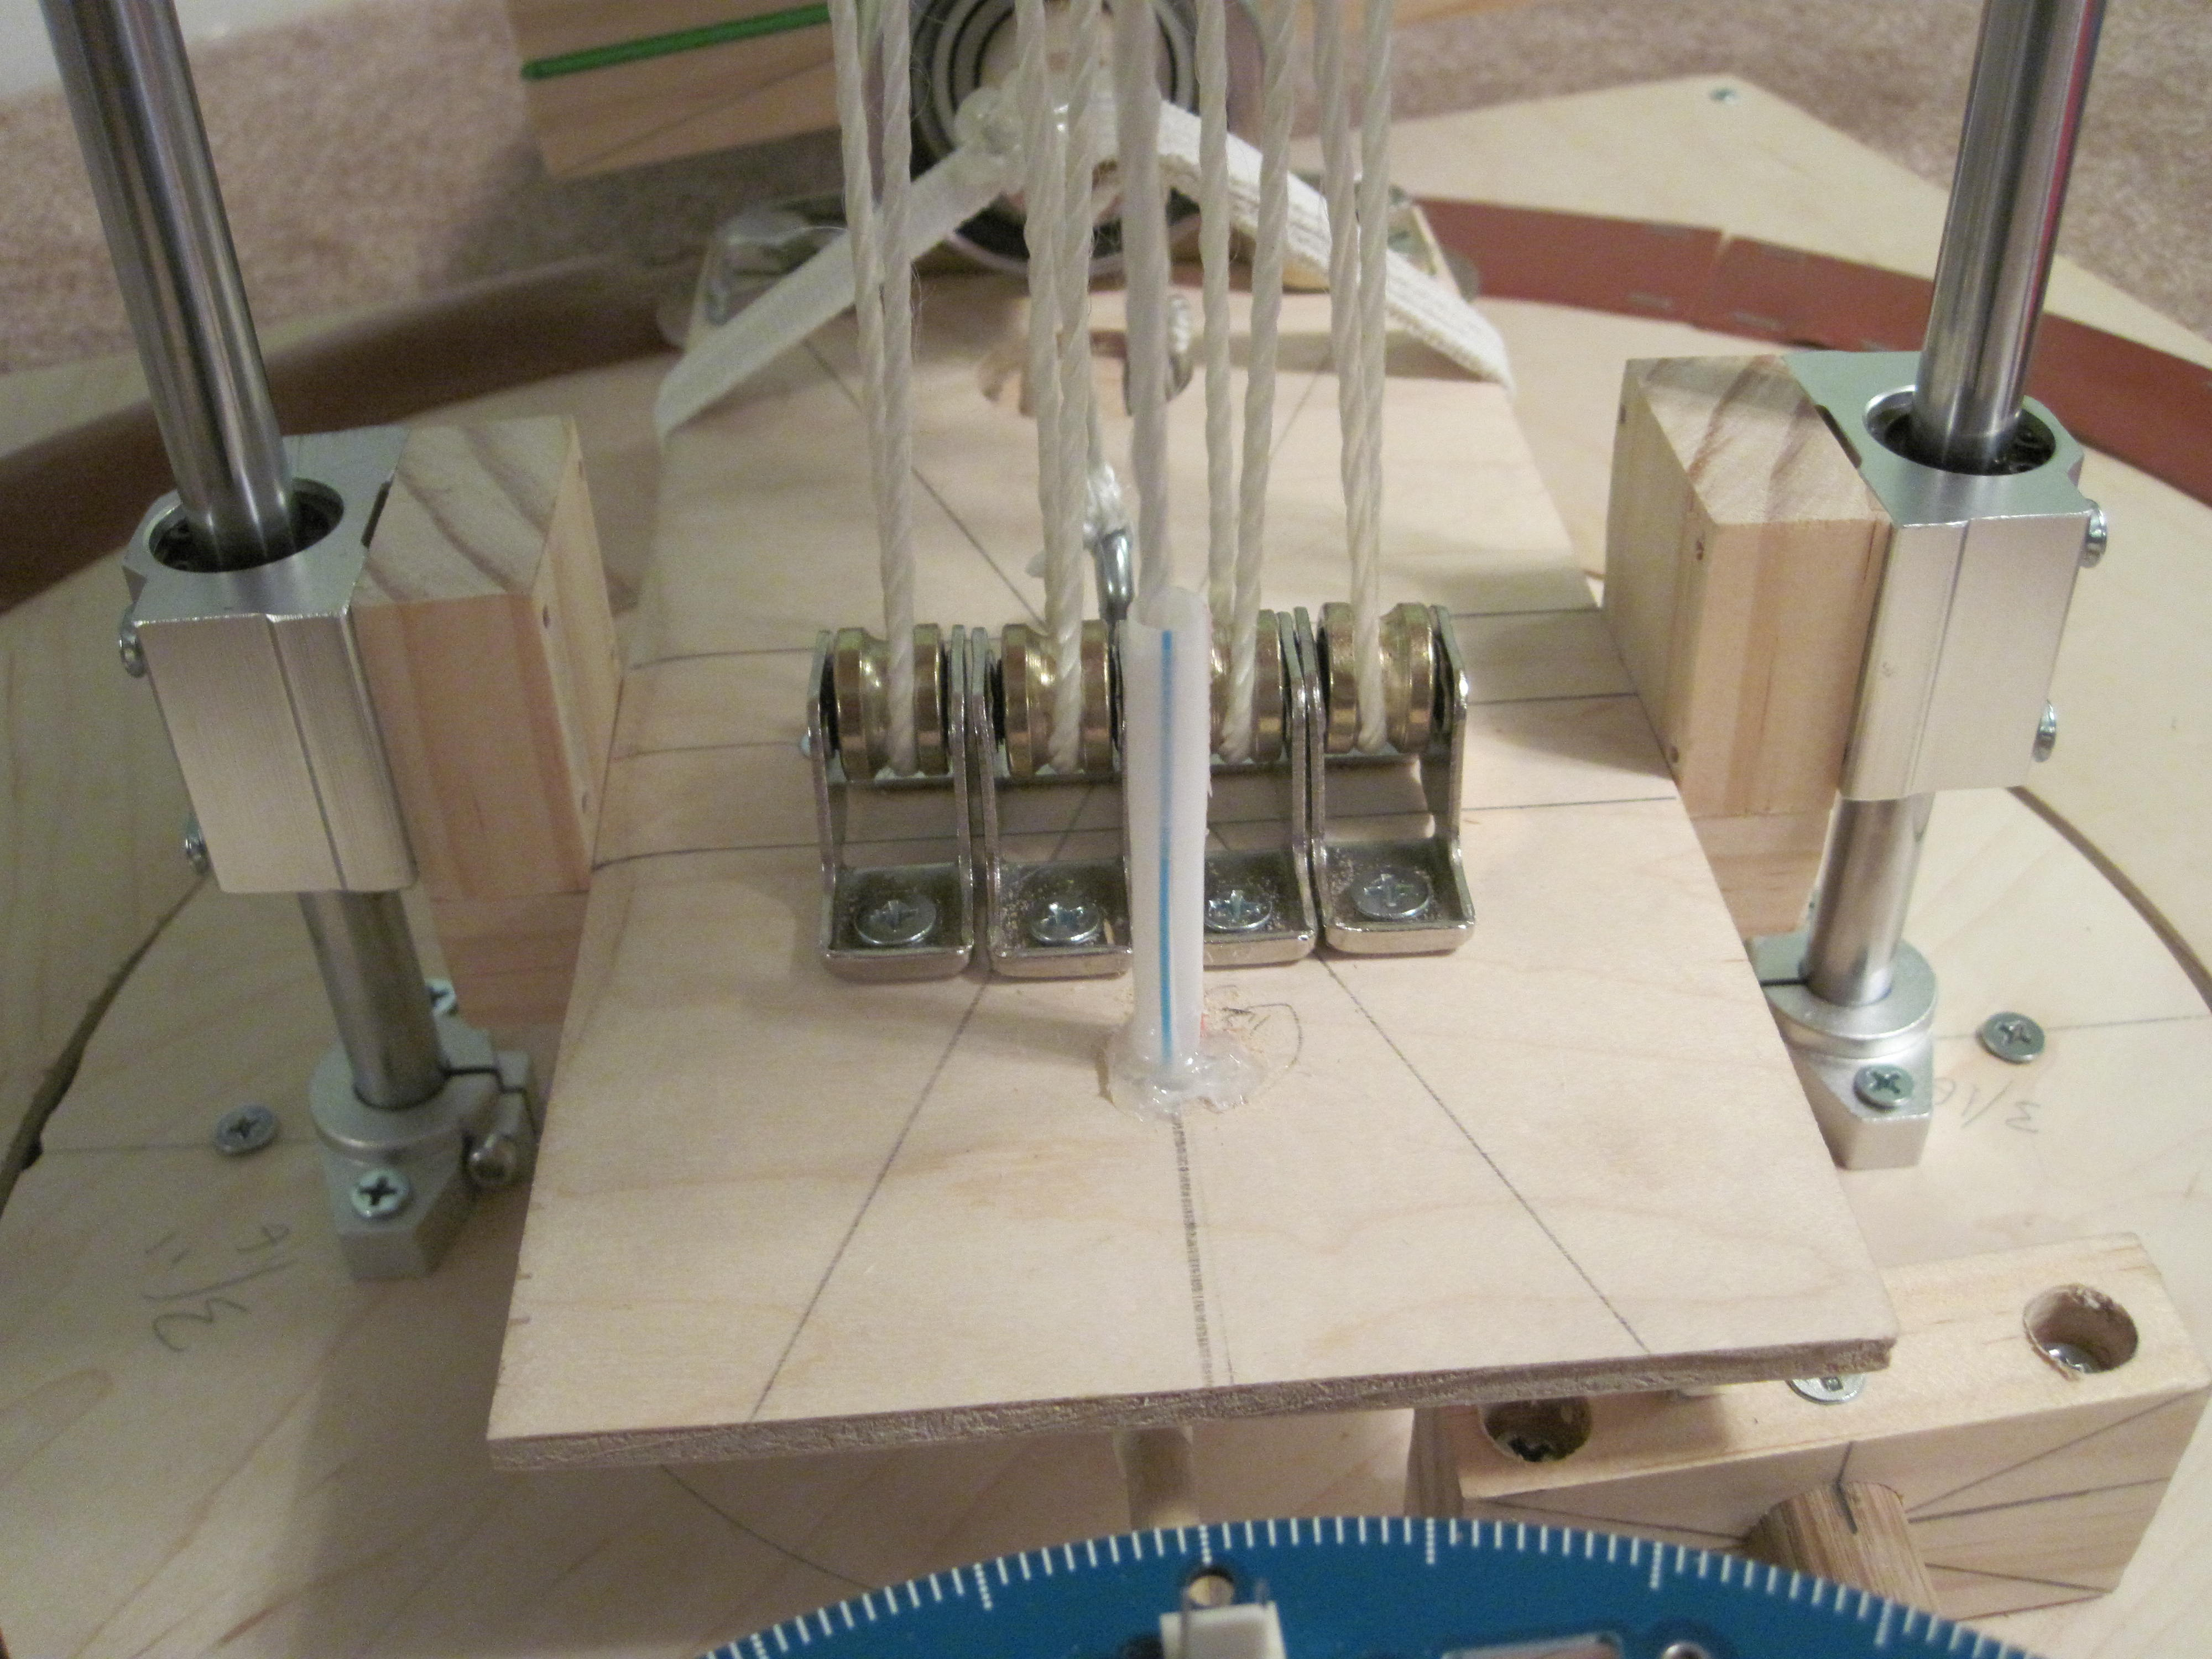
\includegraphics[width=\columnwidth]{Linear Bearings.jpg}
    \caption{The linear bearings.}
    \label{linearbearings}
\end{figure}
\begin{figure}[ht]
  \centering
    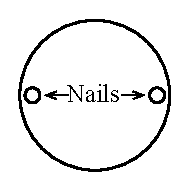
\includegraphics[width=\columnwidth]{Nails.pdf}
    \caption{The location of the nails in the end of the dowel.}
    \label{nails}
\end{figure}
\begin{figure}[ht]
  \centering
3    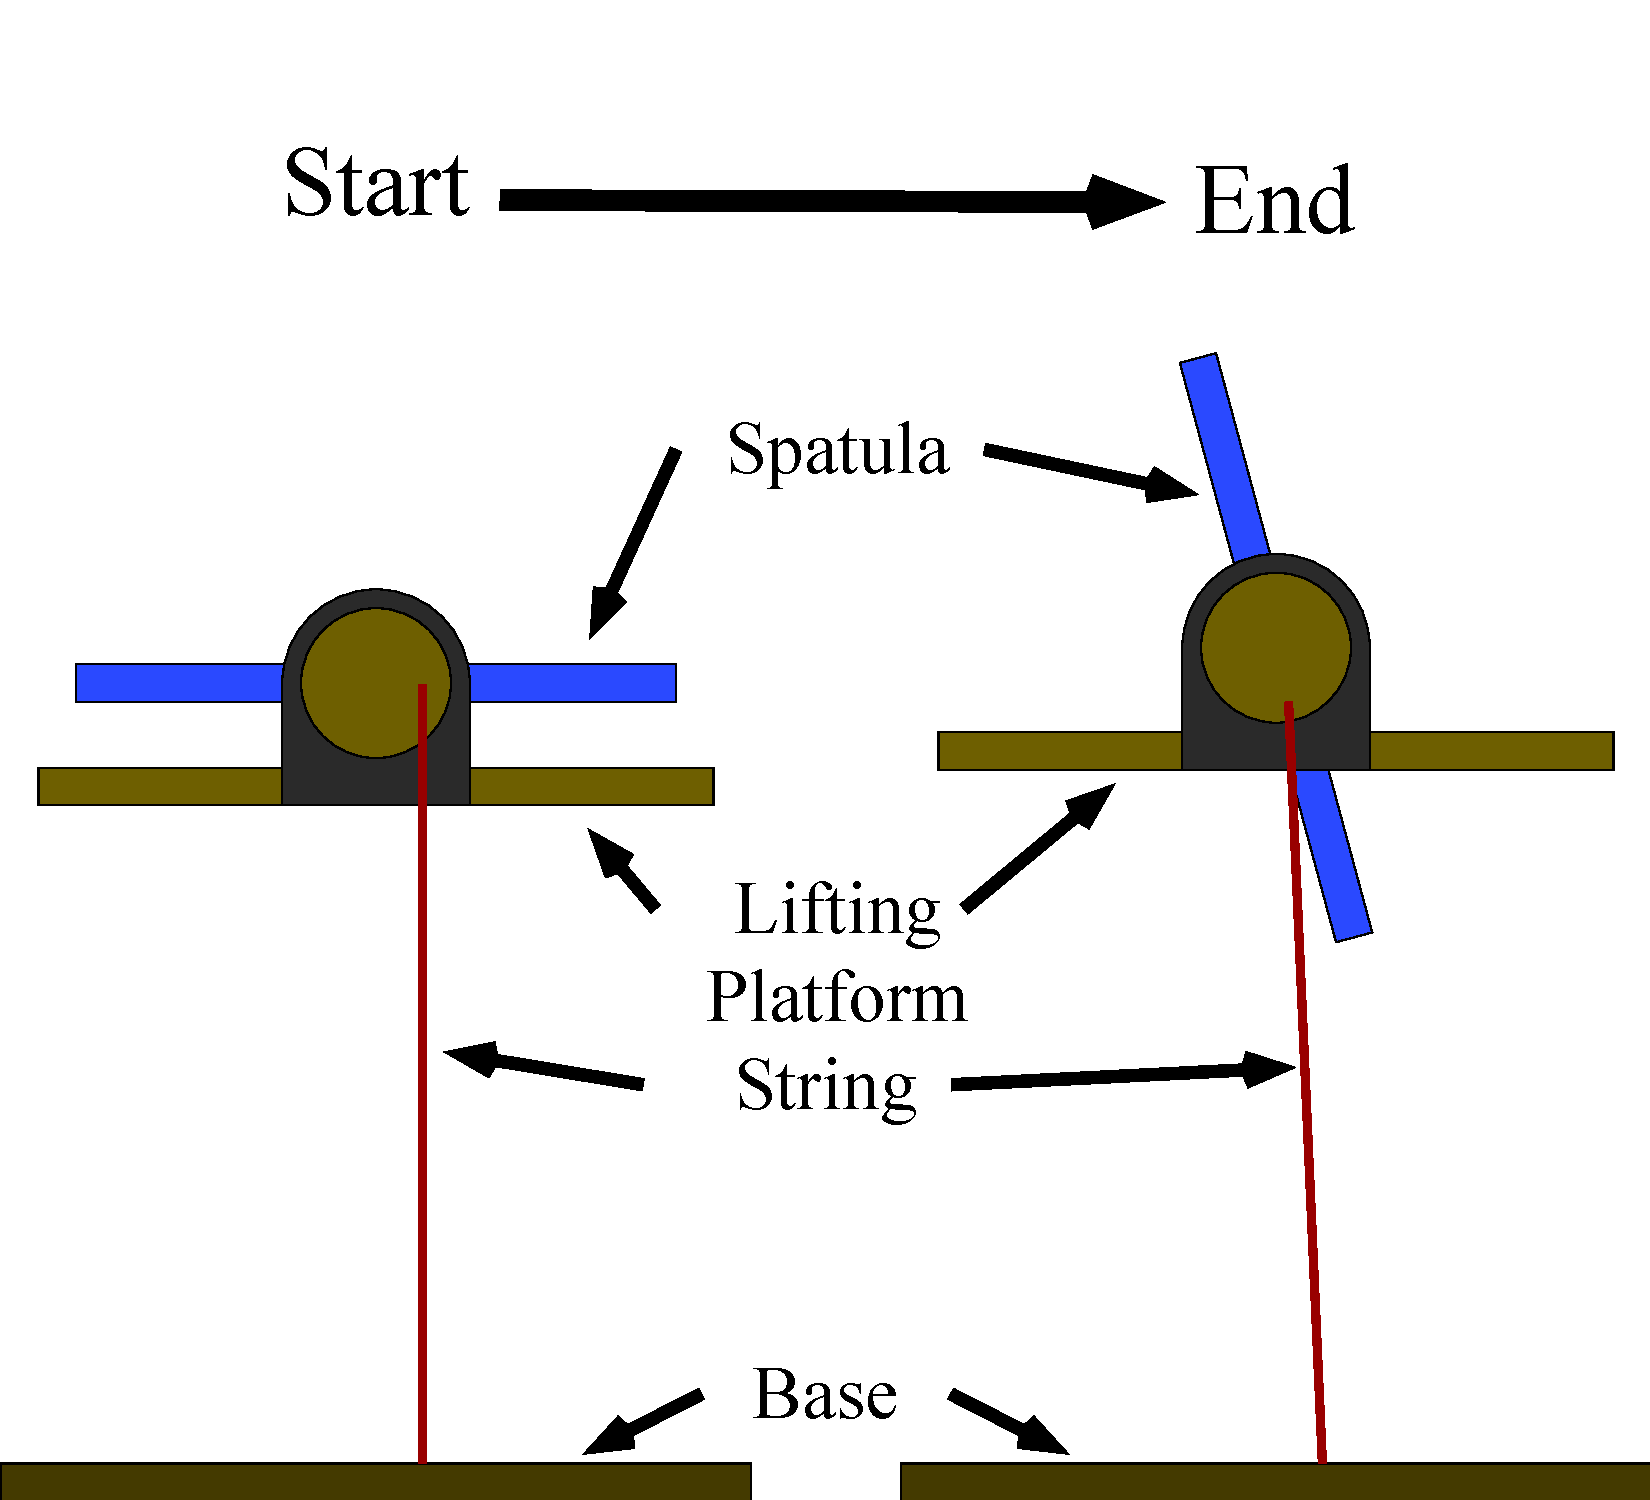
\includegraphics[width=\columnwidth]{Dumping.pdf}
    \caption{The dumping mechanics.}
    \label{dumping}
\end{figure}
\end{document}